\section{Tabular plasticity}

The tabular plasticity model is designed to simulate hypoelastic-plasticity using 
tabulated data for elastic moduli and the yield function for $J_2$ and $J_2-I_1$ models
of perfect plasticity. 

The model has been designed with the high-rate deformation of soils in mind but can 
also be used for non-hardening metals. Sample input files for linear elastic materials
and von Mises plasticity can be found in 
\textsf{src/StandAlone/inputs/MPM/TabularModels/TabularPlasticity}.

\subsection{An input file}
The inputs for the tabular plasticity model are typically specified as follows.
\lstset{
  language=XML
}
\begin{lstlisting}
<?xml version='1.0' encoding='ISO-8859-1' ?>

<Uintah_specification>

  <Meta>
      <title>Tabular_Verification_Test_05_Uniaxial_Strain_Compression_DP_with_LoadUnload</title>
  </Meta>

  <SimulationComponent type="mpm" />

  <Time>
      <maxTime> 8.0 </maxTime>
      <initTime> 0.0 </initTime>
      <delt_min> 1.0e-8 </delt_min>
      <delt_max> 0.01 </delt_max>
      <timestep_multiplier> 0.3 </timestep_multiplier>
  </Time>

  <DataArchiver>
      <filebase>TabularTest_05_UniaxialStrainLoadUnloadNonLinDPNonLin.uda</filebase>
      <outputInterval>1.0e-3</outputInterval>
      <outputInitTimestep/>
      <save label = "p.x"/>
      <save label = "p.color"/>
      <save label = "p.temperature"/>
      <save label = "p.velocity"/>
      <save label = "p.particleID"/>
      <save label = "p.stress"/>
      <save label = "g.mass"/>
      <save label = "p.deformationGradient"/>
      <save label = "g.acceleration"/>
      <save label = "p.plasticVolStrain"/>
      <save label = "p.elasticVolStrain"/>
      <checkpoint cycle = "2" timestepInterval = "2000"/>
  </DataArchiver>

  <MPM>
    <time_integrator>              explicit   </time_integrator>
    <interpolator>                 linear     </interpolator>
    <use_load_curves>              false      </use_load_curves>
    <minimum_particle_mass>        1.0e-15    </minimum_particle_mass>
    <minimum_mass_for_acc>         1.0e-15    </minimum_mass_for_acc>
    <maximum_particle_velocity>    1.0e5      </maximum_particle_velocity>
    <artificial_damping_coeff>     0.0        </artificial_damping_coeff>
    <artificial_viscosity>         true       </artificial_viscosity>
    <artificial_viscosity_heating> false      </artificial_viscosity_heating>
    <do_contact_friction_heating>  false      </do_contact_friction_heating>
    <create_new_particles>         false      </create_new_particles>
    <use_momentum_form>            false      </use_momentum_form>
    <with_color>                   true       </with_color>
    <use_prescribed_deformation>   true       </use_prescribed_deformation>
    <prescribed_deformation_file>  TabularTest_05_PrescribedDeformation.inp   </prescribed_deformation_file>
    <erosion algorithm = "none"/>
  </MPM>

  <PhysicalConstants>
      <gravity>[0,0,0]</gravity>
  </PhysicalConstants>

  <MaterialProperties>
    <MPM>
      <material name="TabularPlastic">
        <density>1050</density>
        <melt_temp>3695.0</melt_temp>
        <room_temp>294.0</room_temp>
        <thermal_conductivity>174.0e-7</thermal_conductivity>
        <specific_heat>134.0e-8</specific_heat>
        <constitutive_model type="tabular_plasticity">
          <elastic_moduli_model type="tabular">
            <filename>TabularTest_05_Elastic.json</filename>
            <independent_variables>PlasticStrainVol, TotalStrainVol</independent_variables>
            <dependent_variables>Pressure</dependent_variables>
            <interpolation type="linear"/>
            <G0>3500</G0>
            <nu>0.35</nu>
          </elastic_moduli_model>
          <plastic_yield_condition type="tabular">
            <filename>TabularTest_05_Yield.json</filename>
            <independent_variables>Pressure</independent_variables>
            <dependent_variables>SqrtJ2</dependent_variables>
            <interpolation type="linear"/>
          </plastic_yield_condition>
        </constitutive_model> 
        <geom_object>
          <box label = "Plate1">
            <min>[0.0,0.0,0.0]</min>
            <max>[1.0,1.0,1.0]</max>
          </box>
          <res>[1,1,1]</res>
          <velocity>[0.0,0.0,0.0]</velocity>
          <temperature>294</temperature>
          <color>0</color>
        </geom_object>
      </material>
      <contact>
        <type>null</type>
        <materials>[0]</materials>
        <mu>0.1</mu>
      </contact>
    </MPM>
  </MaterialProperties>

  <Grid>
      <BoundaryConditions>                      
      </BoundaryConditions>
      <Level>
        <Box label = "1">
            <lower>[-2.0, -2.0, -2.0]</lower>
            <upper>[3.0, 3.0, 3.0]</upper>
            <resolution>[5,5,5]</resolution>
            <extraCells>[0,0,0]</extraCells>
            <patches>[1,1,1]</patches>
        </Box>
      </Level>
  </Grid>

</Uintah_specification>
\end{lstlisting}

\subsubsection{The prescribed deformation file}
The input file listed above is for a single particle driven by a prescribed deformation gradient.  The
deformation file is \textsf{TabularTest\_05\_PrescribedDeformation.inp} which contains the following:
\lstset{
  language=XML
}
\begin{lstlisting}
0  1.0  0  0  0  1  0  0  0  1  0  0  0  0
1  3.0  0  0  0  1  0  0  0  1  0  0  0  0  
3  1.0  0  0  0  1  0  0  0  1  0  0  0  0
5  0.5  0  0  0  1  0  0  0  1  0  0  0  0
7  1.0  0  0  0  1  0  0  0  1  0  0  0  0
8  1.02 0  0  0  1  0  0  0  1  0  0  0  0 
\end{lstlisting}
The first column is the time (seconds), the second column is deformation gradient $F_{xx}$.  This
deformation represents uniaxial strain in the $x$-direction.

\subsubsection{The bulk-modulus model}
The bulk modulus model is non-linear (\textsf{tanh}) and in input as JSON file containing data
that covers the range expected during a simulation.  A sample file  
(\textsf{TabularTest\_05\_Elastic.json}) is shown below:
\lstset{
  language=JSON
}
\begin{lstlisting}
{"Vaango_tabular_data": {
  "Meta" : {
    "title" : "Nonlinear elastic data"
  },
  "Data" : {
    "PlasticStrainVol" : [-2.5, 2.5],
    "Data" : [{
      "TotalStrainVol" : [-15.000000, -14.310345, -13.620690, -12.931034, -12.241379, -11.551724, -10.862069, -10.172414, -9.482759, -8.793103, -8.103448, -7.413793, -6.724138, -6.034483, -5.344828, -4.655172, -3.965517, -3.275862, -2.586207, -1.896552, -1.206897, -0.517241, 0.172414, 0.862069, 1.551724, 2.241379, 2.931034, 3.620690, 4.310345, 5.000000],
      "Pressure" : [-2959.842894, -2943.464146, -2920.494168, -2888.366995, -2843.600634, -2781.548344, -2696.156593, -2579.811517, -2423.426002, -2217.004505, -1950.975669, -1618.496214, -1218.556435, -759.014896, -257.981931, 257.981931, 759.014896, 1218.556435, 1618.496214, 1950.975669, 2217.004505, 2423.426002, 2579.811517, 2696.156593, 2781.548344, 2843.600634, 2888.366995, 2920.494168, 2943.464146, 2959.842894]
    }, {
      "TotalStrainVol" : [-5.000000, -4.310345, -3.620690, -2.931034, -2.241379, -1.551724, -0.862069, -0.172414, 0.517241, 1.206897, 1.896552, 2.586207, 3.275862, 3.965517, 4.655172, 5.344828, 6.034483, 6.724138, 7.413793, 8.103448, 8.793103, 9.482759, 10.172414, 10.862069, 11.551724, 12.241379, 12.931034, 13.620690, 14.310345, 15.000000],
      "Pressure" : [-2959.842894, -2943.464146, -2920.494168, -2888.366995, -2843.600634, -2781.548344, -2696.156593, -2579.811517, -2423.426002, -2217.004505, -1950.975669, -1618.496214, -1218.556435, -759.014896, -257.981931, 257.981931, 759.014896, 1218.556435, 1618.496214, 1950.975669, 2217.004505, 2423.426002, 2579.811517, 2696.156593, 2781.548344, 2843.600634, 2888.366995, 2920.494168, 2943.464146, 2959.842894]
    }]
  }
}}
\end{lstlisting}

\subsubsection{The yield function}
The yield function in this example is a nonlinear Drucker-Prager model.  The input file
(\textsf{TabularTest\_05\_Yield.json}) is shown below:
\lstset{
  language=JSON
}
\begin{lstlisting}
{"Vaango_tabular_data": {
  "Meta" : {
    "title" : "Quadratic Drucker-Prager yield data"
  },
  "Data" : {
    "Pressure" : [-333.333333, -298.850575, -264.367816, -229.885057, -195.402299, -160.919540, -126.436782, -91.954023, -57.471264, -22.988506, 11.494253, 45.977011, 80.459770, 114.942529, 149.425287, 183.908046, 218.390805, 252.873563, 287.356322, 321.839080, 356.321839, 390.804598, 425.287356, 459.770115, 494.252874, 528.735632, 563.218391, 597.701149, 632.183908, 666.666667],
    "SqrtJ2" :   [0.000000, 45.485883, 64.326752, 78.783860, 90.971765, 101.709526, 111.417203, 120.344334, 128.653504, 136.457648, 143.838990, 150.859606, 157.567719, 164.001682, 170.192589, 176.166066,181.943530, 187.543098, 192.980256, 198.268366, 203.419051, 208.442500, 213.347701, 218.142630, 222.834406, 227.429413, 231.933403, 236.351579, 240.688667, 244.948974]
  }
}}
\end{lstlisting}

\subsection{Model components}
Since the tabular plasticity model was designed for materials that have almost no tensile strength,
the inputs are expected in the \textbf{compression positive} convention.  Note that the general
convention used in the Vaango code is that \textbf{tension is positive and compression is negative}.
Conversions are done internally in the code to make sure that signs are consistent.

\begin{SummaryBox}[label=box:TableShearModulusModel]{Shear modulus model}
  The shear modulus is either a constant ($G_0$) or determined using a Poisson's ratio ($\nu$)
  from the tabular bulk modulus, $K(p)$, using a linear elastic model:
  \Beq
    G = \frac{3K(1-2\nu)}{2(1+\nu)}
  \Eeq
  This relation is activated if $\nu \in [-1.0, 0.5)$, otherwise the constant shear modulus
  is used.
\end{SummaryBox}

\begin{SummaryBox}[label=box:TableBulkModulusModel]{Bulk modulus model}
  \begin{center}
    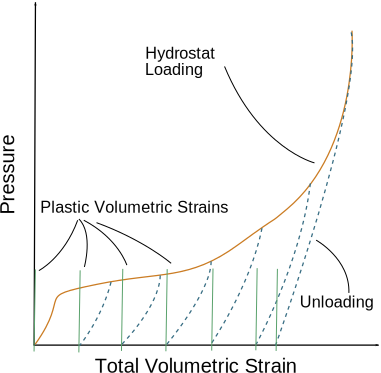
\includegraphics[width=0.5\textwidth]{MPMMaterials/FIGS/TabularHydrostat.pdf}
  \end{center}

  The bulk modulus is determined from a table of unloading curves.  Each unloading 
  curve is associated with a Hencky plastic volumetric strain ($\bar{\Veps_v^p}$).
  These strains are associated in the JSON file with the key \textsf{PlasticStrainVol}
  and added as the first independent variable in the Vaango \textsf{ups} input file.

  For each plastic strain value, the JSON file has to contain an associated data
  set of \textsf{TotalStrainVol} (the total Hencky volumetric strain, $\bar{\Veps_v}$)
  and the \textsf{Pressure} (the mean stress, $\bar{p}$).
\end{SummaryBox}

\begin{SummaryBox}[label=box:TableYieldFunction]{Yield function}
  The tabular yield condition is
  \Beq
     f = \sqrt{J_2} - g(\pbar) = 0
  \Eeq
  \begin{center}
    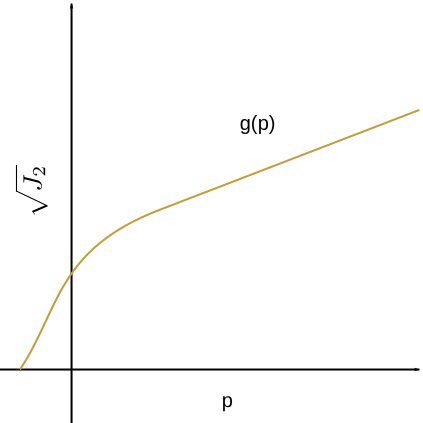
\includegraphics[width=0.4\textwidth]{MPMMaterials/FIGS/TabularYieldFn.pdf}
  \end{center}
  The function $g(\pbar)$ is provided in tabular form.  Only one such function is
  allowed.  The independent variable in the associated JSON file will have the name
  \textsf{Pressure} while the dependent variable will have the name \textsf{SqrtJ2}.
\end{SummaryBox}

\subsection{Examples}
Several examples of input files for exercising various features of the
\Textsfc{TabularPlasticity} model can be found in the directory
\Textsfc{StandAlone/inputs/MPM/TabularModels/TabularPlasticity}.

\subsubsection{von Mises plasticity with linear elasticity compression with rotation}
The input file is \Textsfc{TabularTest\_01\_UniaxialStrainRotateJ2Lin.ups}.
For this problem, $g(\pbar) = \sigma_y$ and $K, G$ are constant. The 
input JSON file for the bulk modulus model is
\begin{lstlisting}[language=JSON]
{"Vaango_tabular_data": {
  "Meta" : {
    "title" : "Test linear elastic data"
  },
  "Data" : {
    "PlasticStrainVol" : [-10.0, 10.0],
    "Data" : [{
      "TotalStrainVol" : [-20.0, 20.0],
      "Pressure" : [-1.0e5,  1.0e5]
    }, {
      "TotalStrainVol" : [-20.0, 20.0],
      "Pressure" : [-1.0e5, 1.0e5]
    }]
  }
}}
\end{lstlisting}
and that for the yield function is
\begin{lstlisting}[language=JSON]
{"Vaango_tabular_data": {
  "Meta" : {
    "title" : "Test von Mises yield data"
  },
  "Data" : {
    "Pressure" : [-0.1e10,  0.1e10],
    "SqrtJ2" :   [  1.0e3,  1.0e3]
  }
}}
\end{lstlisting}
We drive the simulation using uniaxial strain with rotation using the
prescribed deformation file
\begin{lstlisting}[language=sh, backgroundcolor=\color{background}]
0.0   1.000  0.0  0.0   0.0  1.0  0.0   0.0  0.0  1.0    0    0 0 1
1.0   0.900  0.0  0.0   0.0  1.0  0.0   0.0  0.0  1.0   360   0 0 1
\end{lstlisting}
After running the simulation, we get the response shown in Figure~\ref{fig:J2LinRot}.
\begin{figure}[htbp!]
  \begin{subfigure}{0.5\textwidth}
    \centering
    \includegraphics[width=\textwidth]{MPMMaterials/FIGS/UniaxialStrainRotateJ2Lin_yield_surface.pdf}
    \caption{Stress state and yield surface.}
  \end{subfigure}
  \begin{subfigure}{0.5\textwidth}
    \centering
    \includegraphics[width=\textwidth]{MPMMaterials/FIGS/UniaxialStrainRotateJ2Lin_sigma_rot_time.pdf}
    \caption{Rotated stress-time curve.}
  \end{subfigure}
  \begin{subfigure}{0.5\textwidth}
    \centering
    \includegraphics[width=\textwidth]{MPMMaterials/FIGS/UniaxialStrainRotateJ2Lin_pq_time.pdf}
    \caption{Mean and deviatoric stress.}
  \end{subfigure}
  \begin{subfigure}{0.5\textwidth}
    \centering
    \includegraphics[width=\textwidth]{MPMMaterials/FIGS/UniaxialStrainRotateJ2Lin_sigma_time.pdf}
    \caption{Unrotated stress-time curve.}
  \end{subfigure}
  \caption{Stress evolution for $J_2$ plasticity with linear elasticity under uniaxial
           strain compression with rotation.}
  \label{fig:J2LinRot}
\end{figure}

\newpage
\subsubsection{von Mises plasticity with linear elasticity loading-unloading} 
If we change the prescribed deformation to loading-unloading, using the input 
deformation
\begin{lstlisting}[language=sh, backgroundcolor=\color{background}]
0  1.0  0  0  0  1  0  0  0  1  0  0  0  0
1  1.15  0  0  0  1  0  0  0  1  0  0  0  0
3  1.0  0  0  0  1  0  0  0  1  0  0  0  0
5  0.85  0  0  0  1  0  0  0  1  0  0  0  0
7  1.0  0  0  0  1  0  0  0  1  0  0  0  0
8  1.02 0  0  0  1  0  0  0  1  0  0  0  0
\end{lstlisting}
we get the response shown in Figure~\ref{fig:J2LinLoadUnload}
\begin{figure}[htbp!]
  \begin{subfigure}{0.5\textwidth}
    \centering
    \includegraphics[width=\textwidth]{MPMMaterials/FIGS/UniaxialStrainLoadUnloadJ2Lin_yield_surface.pdf}
    \caption{Stress state and yield surface.}
  \end{subfigure}
  \begin{subfigure}{0.5\textwidth}
    \centering
    \includegraphics[width=\textwidth]{MPMMaterials/FIGS/UniaxialStrainLoadUnloadJ2Lin_pq_time.pdf}
    \caption{Mean and deviatoric stress vs. time.}
  \end{subfigure}
  \begin{subfigure}{0.5\textwidth}
    \centering
    \includegraphics[width=\textwidth]{MPMMaterials/FIGS/UniaxialStrainLoadUnloadJ2Lin_sigma_time.pdf}
    \caption{Stress versus time.}
  \end{subfigure}
  \caption{Stress evolution for $J_2$ plasticity with linear elasticity under uniaxial strain
           loading and unloading.}
  \label{fig:J2LinLoadUnload}
\end{figure}

\newpage
\subsubsection{von Mises plasticity with nonlinear elasticity loading-unloading} 
If we replace the linear elastic model with a nonlinear one:
\begin{lstlisting}[language=JSON]
{"Vaango_tabular_data": {
  "Meta" : {
    "title" : "Test nonlinear elastic data"
  },
  "Data" : {
    "PlasticStrainVol" : [-0.02, 0.02],
    "Data" : [{
      "TotalStrainVol" : [-0.295000, -0.276034, -0.257069, -0.238103, -0.219138, -0.200172, -0.181207, -0.162241, -0.143276, -0.124310, -0.105345, -0.086379, -0.067414, -0.048448, -0.029483, -0.010517, 0.008448,0.027414, 0.046379, 0.065345, 0.084310, 0.103276, 0.122241, 0.141207, 0.160172, 0.179138, 0.198103, 0.217069, 0.236034, 0.255000],
      "Pressure" : [-3000.000000, -2982.413871, -2929.861667, -2842.959514, -2722.726259, -2570.571529, -2388.279197, -2177.986476, -1942.158854, -1683.561196, -1405.225322, -1110.414466, -802.585016, -485.345990, -162.416726, 162.416726, 485.345990, 802.585016, 1110.414466, 1405.225322, 1683.561196, 1942.158854, 2177.986476, 2388.279197, 2570.571529, 2722.726259, 2842.959514, 2929.861667, 2982.413871, 3000.000000]
    }, {
      "TotalStrainVol" : [-0.255000, -0.236034, -0.217069, -0.198103, -0.179138, -0.160172, -0.141207, -0.122241, -0.103276, -0.084310, -0.065345, -0.046379, -0.027414, -0.008448, 0.010517, 0.029483, 0.048448, 0.067414, 0.086379, 0.105345, 0.124310, 0.143276, 0.162241, 0.181207, 0.200172, 0.219138, 0.238103, 0.257069, 0.276034, 0.295000],
      "Pressure" : [-3000.000000, -2982.413871, -2929.861667, -2842.959514, -2722.726259, -2570.571529, -2388.279197, -2177.986476, -1942.158854, -1683.561196, -1405.225322, -1110.414466, -802.585016, -485.345990, -162.416726, 162.416726, 485.345990, 802.585016, 1110.414466, 1405.225322, 1683.561196, 1942.158854, 2177.986476, 2388.279197, 2570.571529, 2722.726259, 2842.959514, 2929.861667, 2982.413871, 3000.000000]
    }]
  }
}}
\end{lstlisting}
we get the response shown in Figure~\ref{fig:J2NonLinLoadUnload}
\begin{figure}[htbp!]
  \begin{subfigure}{0.5\textwidth}
    \centering
    \includegraphics[width=\textwidth]{MPMMaterials/FIGS/UniaxialStrainLoadUnloadJ2NonLin_yield_surface.pdf}
    \caption{Stress state and yield surface.}
  \end{subfigure}
  \begin{subfigure}{0.5\textwidth}
    \centering
    \includegraphics[width=\textwidth]{MPMMaterials/FIGS/UniaxialStrainLoadUnloadJ2NonLin_sigma_eps.pdf}
    \caption{Stress vs. strain.}
  \end{subfigure}
  \begin{subfigure}{0.5\textwidth}
    \centering
    \includegraphics[width=\textwidth]{MPMMaterials/FIGS/UniaxialStrainLoadUnloadJ2NonLin_pq_time.pdf}
    \caption{Mean and deviatoric stress vs. time.}
  \end{subfigure}
  \begin{subfigure}{0.5\textwidth}
    \centering
    \includegraphics[width=\textwidth]{MPMMaterials/FIGS/UniaxialStrainLoadUnloadJ2NonLin_sigma_time.pdf}
    \caption{Stress versus time.}
  \end{subfigure}
  \caption{Stress evolution for $J_2$ plasticity with nonlinear elasticity under uniaxial strain
           loading and unloading.}
  \label{fig:J2NonLinLoadUnload}
\end{figure}

\newpage
\subsubsection{Linear Drucker-Prager plasticity with nonlinear elasticity loading-unloading} 
If we change the yield function to a linear Drucker-Prager type model:
\begin{lstlisting}[language=JSON]
{"Vaango_tabular_data": {
  "Meta" : {
    "title" : "Test linear Drucker-Prager yield data"
  },
  "Data" : {
    "Pressure" : [-0.1e3,  0.1e10],
    "SqrtJ2" :   [  0,  3.0e8]
  }
}}
\end{lstlisting}
and use the nonlinear elastic model:
\begin{lstlisting}[language=JSON]
{"Vaango_tabular_data": {
  "Meta" : {
    "title" : "Test nonlinear elastic data"
  },
  "Data" : {
    "PlasticStrainVol" : [-2.5, 2.5],
    "Data" : [{
      "TotalStrainVol" : [-15.000000, -14.310345, -13.620690, -12.931034, -12.241379, -11.551724, -10.862069, -10.172414, -9.482759, -8.793103, -8.103448, -7.413793, -6.724138, -6.034483, -5.344828, -4.655172, -3.965517, -3.275862, -2.586207, -1.896552, -1.206897, -0.517241, 0.172414, 0.862069, 1.551724, 2.241379, 2.931034, 3.620690, 4.310345, 5.000000],
      "Pressure" : [-2959.842894, -2943.464146, -2920.494168, -2888.366995, -2843.600634, -2781.548344, -2696.156593, -2579.811517, -2423.426002, -2217.004505, -1950.975669, -1618.496214, -1218.556435, -759.014896, -257.981931, 257.981931, 759.014896, 1218.556435, 1618.496214, 1950.975669, 2217.004505, 2423.426002, 2579.811517, 2696.156593, 2781.548344, 2843.600634, 2888.366995, 2920.494168, 2943.464146, 2959.842894]
    }, {
      "TotalStrainVol" : [-5.000000, -4.310345, -3.620690, -2.931034, -2.241379, -1.551724, -0.862069, -0.172414, 0.517241, 1.206897, 1.896552, 2.586207, 3.275862, 3.965517, 4.655172, 5.344828, 6.034483, 6.724138, 7.413793, 8.103448, 8.793103, 9.482759, 10.172414, 10.862069, 11.551724, 12.241379, 12.931034, 13.620690, 14.310345, 15.000000],
      "Pressure" : [-2959.842894, -2943.464146, -2920.494168, -2888.366995, -2843.600634, -2781.548344, -2696.156593, -2579.811517, -2423.426002, -2217.004505, -1950.975669, -1618.496214, -1218.556435, -759.014896, -257.981931, 257.981931, 759.014896, 1218.556435, 1618.496214, 1950.975669, 2217.004505, 2423.426002, 2579.811517, 2696.156593, 2781.548344, 2843.600634, 2888.366995, 2920.494168, 2943.464146, 2959.842894]
    }]
  }
}}
\end{lstlisting}
we get the response shown in Figure~\ref{fig:DPNonLinLoadUnload}
\begin{figure}[htbp!]
  \begin{subfigure}{0.5\textwidth}
    \centering
    \includegraphics[width=\textwidth]{MPMMaterials/FIGS/UniaxialStrainLoadUnloadDPNonLin_yield_surface.pdf}
    \caption{Stress state and yield surface.}
  \end{subfigure}
  \begin{subfigure}{0.5\textwidth}
    \centering
    \includegraphics[width=\textwidth]{MPMMaterials/FIGS/UniaxialStrainLoadUnloadDPNonLin_sigma_eps.pdf}
    \caption{Stress vs. strain.}
  \end{subfigure}
  \begin{subfigure}{0.5\textwidth}
    \centering
    \includegraphics[width=\textwidth]{MPMMaterials/FIGS/UniaxialStrainLoadUnloadDPNonLin_pq_time.pdf}
    \caption{Mean and deviatoric stress vs. time.}
  \end{subfigure}
  \begin{subfigure}{0.5\textwidth}
    \centering
    \includegraphics[width=\textwidth]{MPMMaterials/FIGS/UniaxialStrainLoadUnloadDPNonLin_sigma_time.pdf}
    \caption{Stress versus time.}
  \end{subfigure}
  \caption{Stress evolution for Drucker-Prager plasticity with nonlinear elasticity under uniaxial strain
           loading and unloading.}
  \label{fig:DPNonLinLoadUnload}
\end{figure}

\newpage
\subsubsection{Nonlinear Drucker-Prager plasticity with nonlinear elasticity loading-unloading} 
Finally, if we change the yield function to a nonlinear Drucker-Prager type model:
\begin{lstlisting}[language=JSON]
{"Vaango_tabular_data": {
  "Meta" : {
    "title" : "Test nonlinear Drucker-Prager yield data"
  },
  "Data" : {
    "Pressure" : [-333.333333, -298.850575, -264.367816, -229.885057, -195.402299, -160.919540, -126.436782, -91.954023, -57.471264, -22.988506, 11.494253, 45.977011, 80.459770, 114.942529, 149.425287, 183.908046, 218.390805, 252.873563, 287.356322, 321.839080, 356.321839, 390.804598, 425.287356, 459.770115, 494.252874, 528.735632, 563.218391, 597.701149, 632.183908, 666.666667],
    "SqrtJ2" :   [0.000000, 45.485883, 64.326752, 78.783860, 90.971765, 101.709526, 111.417203, 120.344334, 128.653504, 136.457648, 143.838990, 150.859606, 157.567719, 164.001682, 170.192589, 176.166066,181.943530, 187.543098, 192.980256, 198.268366, 203.419051, 208.442500, 213.347701, 218.142630, 222.834406, 227.429413, 231.933403, 236.351579, 240.688667, 244.948974]
  }
}}
\end{lstlisting}
we get the response shown in Figure~\ref{fig:NonLinDPNonLinLoadUnload}
\begin{figure}[htbp!]
  \begin{subfigure}{0.5\textwidth}
    \centering
    \includegraphics[width=\textwidth]{MPMMaterials/FIGS/UniaxialStrainLoadUnloadNonLinDPNonLin_yield_surface.pdf}
    \caption{Stress state and yield surface.}
  \end{subfigure}
  \begin{subfigure}{0.5\textwidth}
    \centering
    \includegraphics[width=\textwidth]{MPMMaterials/FIGS/UniaxialStrainLoadUnloadNonLinDPNonLin_sigma_eps.pdf}
    \caption{Stress vs. strain.}
  \end{subfigure}
  \begin{subfigure}{0.5\textwidth}
    \centering
    \includegraphics[width=\textwidth]{MPMMaterials/FIGS/UniaxialStrainLoadUnloadNonLinDPNonLin_pq_time.pdf}
    \caption{Mean and deviatoric stress vs. time.}
  \end{subfigure}
  \begin{subfigure}{0.5\textwidth}
    \centering
    \includegraphics[width=\textwidth]{MPMMaterials/FIGS/UniaxialStrainLoadUnloadNonLinDPNonLin_sigma_time.pdf}
    \caption{Stress versus time.}
  \end{subfigure}
  \caption{Stress evolution for Drucker-Prager plasticity with nonlinear elasticity under uniaxial strain
           loading and unloading.}
  \label{fig:NonLinDPNonLinLoadUnload}
\end{figure}
